\chapter{Symmetry in \pCf}	
\epigraph{Tyger! Tyger! Burning bright, \\
		In the forests of the night. \\
		What immortal hand or eye,\\
		Could frame thy fearful symmetry?}{William Blake, \emph{The Tyger}} 
The dynamcal behavior of a physical system often displays symmetry. The electron wavefunction in the ground state of hydrogen, or the gravitational motion of a planet around a star, for instance, display very high degrees of spatial symmetry.  Understanding the symmetries of a system can be incredibly useful to an investigator, since they hint at conserved physical quantities (through Noether's Theorem), and can greatly reduce the complexity of the system in various ways. In order to further discuss symmetry, it will be useful to introduce some terminology, following the conventions in\cite{Rotman1995}.  \\

\begin{define}
A {\bf group} $(G,\ast)$ is an object that contains a set $G$ and a binary operator known as the {\bf group law} $\ast: G \times G \to G$ that has the following properties 
\begin{enumerate}
\item {\bf Closure}: For every $a,b\in G$, $a \ast b \in G$,
\item {\bf Associativity}: For every $a,b,c \in G$, $a \ast (b\ast c) = (a\ast b)\ast c$,
\item {\bf Identity}: There exists a so-called identity $e \in G$ such that for any $a \in G$, $e\ast a = a$,
\item {\bf Inverse}: For all $a\in G$, there exists an inverse $a^{-1} \in G$ such that $a \ast a^{-1}=a^{-1}\ast a = e$.
\end{enumerate}
and has a group action $\star: G\times A \to A$ on a set $A$ such that 
\begin{enumerate}
\item {\bf Associativity} For all $a,b \in G$ and $\alpha \in A$, $a\star(b\star\alpha) =  (a \ast b)\star \alpha$,
\item {\bf Identity} For all $\alpha \in A$, $e \star \alpha = \alpha$.
\end{enumerate}
\end{define}
\clearpage
\begin{define}
The {\bf order} of a group $(G,\ast)$ is the number of elements in $G$. 
\end{define}
\begin{define}
A {\bf subgroup} $(H,\ast)$ of $(G,\ast)$ is a group such that $H \subseteq G$.  
\end{define}
\begin{define}
A {\bf dynamical system} is an object $(R,X,T)$, where $X$ is the state space, $T$ is a set of times, and $R: X \times T \rightarrow X$ is a function that describes how a state evolves in time. That is, $x' = R_t(x) \in X$ describes the state that the inital condition $x \in X$ evolves to after a time $t \in T$. If $X$ and $f$ are continuously differentiable with time, then
\begin{equation}
\pder{1}{}{t}R_t(x) |_{t=0} = f(x),
\end{equation} 
 so that the set of points an initial condition evolves through (known as the {\bf trajectory}) is described by the ordinary differential equation (ODE)
\begin{equation}
\der{1}{x}{t} = f(x).
\end{equation}
I will refer to a dynamical system by its ODE, with the understanding that it applies to all $x \in X$. 
\end{define}
\begin{define}\label{def:equivariance}
A {\bf symmetry group} for a dynamical system $\dot{\Vector{x}} = \Vector{f}(\Vector{x})$  is the group $(\Sigma,\ast)$ such that for any linear transformation $\sigma \in \Sigma$, 
\begin{equation}
\sigma\star \dot{\Vector{x}} = \sigma\star \Vector{f}(\Vector{x}) = \Vector{f}(\sigma \star \Vector{x}).
\end{equation}
Such a linear transformation is said to be a symmetry transformation, and the dynamical system is then said to be {\bf $\Sigma$-equivariant}.
\end{define}
\begin{define}
For a particular state $\Vector{u}$ in a dynamical system $\dot{\Vector{x}} = \Vector{f}(\Vector{x})$ , a symmetry group $(\Sigma,\ast)$ such that for all $\sigma \in \Sigma$,
\begin{equation}
\sigma \Vector{u}  = \Vector{u}
\end{equation}
is known as the {\bf isotropy subgroup} of $\Vector{u}$, and $\Vector{u}$ is said to {\bf satisfy} or be {\bf fixed} by $\Sigma$. 
\end{define}
\begin{define}
If a group $(G,\ast)$ has the further property that for all $a,b \in G$, $a \ast b = b \ast a$, then the group is {\bf abelian}
\end{define}
\begin{define}\label{def:conjugacy}
Two subgroups $(J,\ast)$ and $(H,\ast)$ of $(G,\ast)$ are considered {\bf conjugate} if for some $a \in G$,
\begin{equation}
a\ast J \ast a^{-1} = H.
\end{equation} 
A set of mutually conjugate groups makes up a {\bf conjugacy class}, and since the action of members of a conjugacy class on a particular state $\Vector{u}$ can be considered equivalent\footnote{Since conjugate groups are essentially related by a coordiante transformation\rf{GIBSON2009}}, only one representative member of a conjugacy class needs to be considered. 
\end{define}
\begin{define}
A set $\mathcal{G}$ is said to {\bf generate} a group $(G,\ast)$ if repeated applications of the group law between elements of $\mathcal{G}$ produces all the elements of $G$.
\end{define}
The symmetry relations of \pCf\ are discussed extensively in\rf{GIBSON2009,Halcrow2008}, which I will present here for the sake of flow.\footnote{haha} To keep notation compact, the group action and group law operator is omitted and can be inferred from context, and a group $(G,\ast)$ is referred to by the set $G$. 
\section{Unbounded Navier-Stokes}

If we do not impose boundary conditions on the 3D Navier-Stokes equations on an infinite domain, the system will be equivariant under the group of continuous rotational and translational symmetry transformations, as well as the discrete {\bf pointwise inversion} symmetry transformation $\sigma_{xz}$\rf{Frisch1995}, which has the following action on the system:

\begin{equation}\label{eq:pointwiseinversion}
\sigma_{xz}\Vector{u}\paren{\Vector{x}} = -\Vector{u}\paren{-\Vector{x}}
\end{equation}

While the rotation or translation transformation can be easily conceptualized, the pointwise inversion transformation can provide some difficulty. The easiest way of visualizing the transformation is to view it in a 2D domain instead of in the full 3D, as shown in \figureref{fig:pointwiseinversion}. 

\begin{figure}[h]
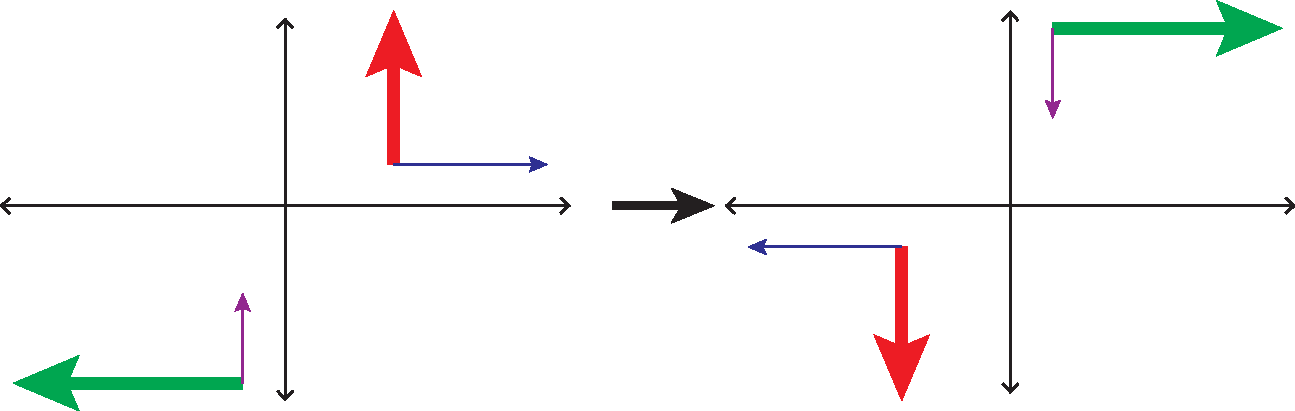
\includegraphics[width=\textwidth]{pointwiseinversion}
\caption{A 2D pointwise inversion operation on two sets of vectors according to \refeq{eq:pointwiseinversion}.}\label{fig:pointwiseinversion}

\end{figure}


\section{Plane Couette Flow}

If the domain is limited to $\mathbb{R}^2 \times [-1,1]$ with the boundary conditions of \pCf, we lose some of the symmetry transformations of the full, unrestricted problem, leaving us with two basic discrete symmetries: a rotation by $\pi$ about the $z$ axis (denoted $\sigma_x$) and a reflection about the $z$ axis (denoted $\sigma_z$)\footnote{The motivation for these subscripts will become apparent shortly.}, together form a discrete symmetry group $D = D_1 \times D_1 = \{e, \sigma_x,\sigma_z,\sigma_{xz}\}$ of order 4, where

\begin{align}\label{eq:discretesymm}
\sigma_x [u,v,w](x,y,z) &= [-u,-v,w](-x,-y,z)\\
\sigma_z [u,v,w](x,y,z) &= [u,v,-w](x,y,-z)\\
\sigma_{xz} [u,v,w](x,y,z) &= [-u,-v,-w](-x,-y,-z)
\end{align}

We also lose the general rotation and translational symmetries, keeping only the two parameter steamwise-spanwise translations. If we then apply periodic boundary conditions, these take the form of a continuous $SO(2)\times SO(2)$ symmetry group 
\begin{align}
\tau_x(l_x)[u,v,w](x,y,z) = [u,v,w](x+l_x,y,z),\label{eq:contsymm}\\
\tau_z(l_z)[u,v,w](x,y,z) = [u,v,w](x,y,z+l_z),\\
\tau_xz[u,v,w](x,y,z) = \tau_x\tau_z[u,v,w](x,y,z).
\end{align}

The complete symmetry group is then any combination of these symmetry operations, given by $\Sigma = SO(2)_x \ltimes D_{1,x} \times SO(2)_z \ltimes D_{1,z}.$\footnote{$\ltimes$ is the semidirect product}
\section{Properties and Isotropy Subgroups of $\Sigma$}

It should be evident that since \pCf\ is equivariant under the continuous translations given in \eqref{eq:contsymm}, solutions can take the form of traveling waves or relative periodic orbits: that is, there exists a different reference frame in which the trajectory is a regular equilibrium or periodic orbit. However, an initial condition that is fixed by $\sigma_z$ cannot be translated in the spanwise direction without losing $\sigma_z$ symmetry (except for the trivial case where $\pder{1}{\Vector{u}_z}{z} = 0$). Similarly, an initial condition that is fixed by $\sigma_x$ cannot be translated in the streamwise direction without losing $\sigma_x$ symmetry (and an initial condition that is fixed by $\sigma_{xz}$ symmetry cannot be translated at all without losing $\sigma_{xz}$ symmetry). Since these symmetries are also invariant,\footnote{That is, if the symmetry is satisfied at time $t = t_0$, it must be satisfied for all times. This is trivially true from \refDef{def:equivariance}.} a trajectory with one of the discrete symmetries cannot be a traveling wave in the direction corresponding to its subscript. \\
 \begin{figure}[t!]
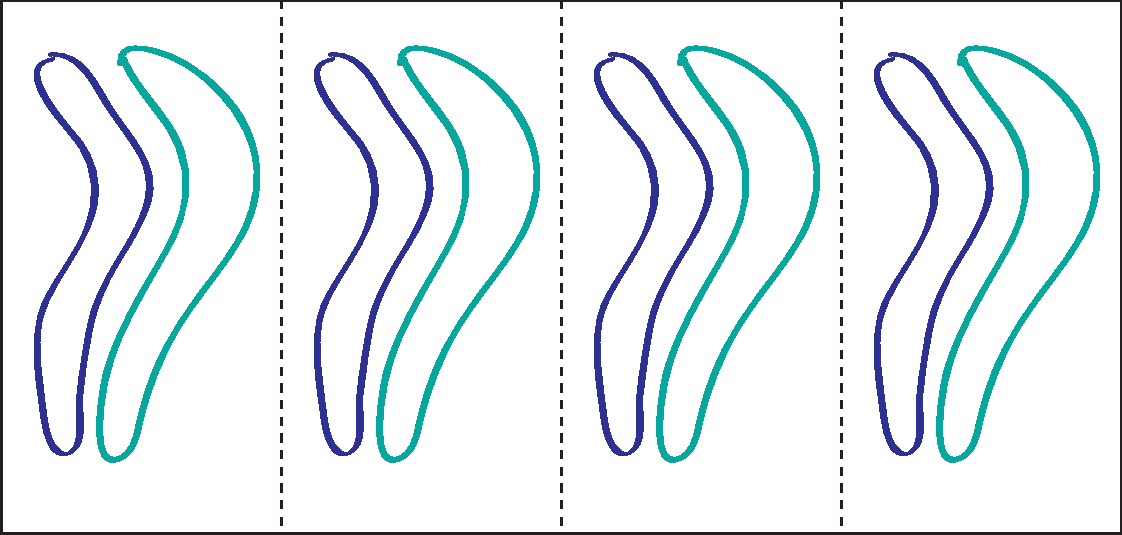
\includegraphics[width=\textwidth]{SubCell}
\caption{If the flow state is fixed by $\tau(\dfrac{1}{4}L_x,0)$, then the solution will have four repeating streamwise subcells, and it becomes more efficient to solely consider the subcell.}\label{fig:rationalTranslation}

\end{figure}
The presence of the periodic boundary conditions also implies that all solutions are fixed by a translation $\tau(L_x,0)$ and $\tau(0,L_z)$ that corresponds to shifting by a whole box length. However, solutions can also be fixed by any rational translation of the form $\tau(a L_x,b L_z)$, where $a,b \in \mathbb{Q}$, or by  continuous translations. If we fix $\Vector{u}$ by a continuous translation, we force it to have a zero derivative along that axis\footnote{That is, if we fix $\Vector{u}$ by $\tau(l_x,0)$ for any real $l_x$, then $\pder{1}{\Vector{u}}{x} = 0$, and similarly for $z$.}, and such solutions tend to be uninteresting as they are equivalent to lower-dimensional problems. If $\Vector{u}$ is fixed instead by rational translations, the periodic cell is tiled with repeating subcells, as in \refFig{fig:rationalTranslation}. This implies that we can restrict ourselves to full box length translations, which are forced on us by the periodic boundary conditions.\\

There is one further reason to restrict the translation symmetry - the unrestricted $\Sigma$ is not an abelian group, as demonstrated in \refFig{fig:notabelian}, so the order in which symmetry transformations are applied matters. This is undesierable, since it makes the classification of groups slightly more complex, especially when trying to sort groups into their conjugacy classes. From \refeqs{eq:discretesymm}{eq:contsymm} however, it is evident that the following relation between the $\sigma$ and $\tau$ holds:
\begin{equation}
\sigma_{i}\tau_{i} = \tau_i^{-1}\sigma_i,
\end{equation}
where $i$ can index the $x$,$z$ or $xz$ symmetries. Right-multiplication by $\tau_i$ yields
\begin{equation}\label{eq:pscom}
\sigma_i\tau_i^2 = \tau_i^{-1}\sigma_i\tau_i.
\end{equation}
If $\tau_i$ is restricted to \emph{half}-box shifts, then \refeq{eq:pscom} becomes
\begin{equation}
\sigma_i\tau_{i,2}^2 = \sigma_i\tau_{i,1} = \sigma_i = \tau_{i,2}^{-1}\sigma_{i}\tau_{i,2},
\end{equation}
where $\tau_{i,n} = \tau_i(L_i/n)$ represents the spatial periodicity imposed by $\tau$. Right multiplication by $\tau_{i,2}$ yields
\begin{equation}
\tau_{i,2}\sigma_{i} = \sigma_{i}\tau_{i,2}.
\end{equation}
So if $\tau$ is restricted to half-integer box shifts, $\Sigma$ becomes $\Sigma_2$, which is an abelian group, as demonstrated in \refFig{fig:abelian}\footnote{Note that this also implies that $\tau_{i,2}$ is its own inverse.}. The subgroups of $\Sigma_2$, which form the isotropy subgroups we consider for \pCf, are of order $\{1,2,4,8,16\}$. There is only one order 1 subgroup: $\{ e \}$, which is the typical isotropy group for turbulent flows\footnote{Since they lack any symmetry.}. There are 15 subgroups of order 2, 35 subgroups of order 4, 15 subgroups of order 8, and one subgroup of order 16, giving 67 subgroups. Luckily, consideration of conjugacy classes greatly lowers the number of subgroups we need to consider. As an example, consider the subgroups $\{ e, \sigma_x\}$ and $\{e, \sigma_x\tau_{x,2}\}$.
\clearpage
\begin{theorem}
The subgroups $\{ e, \sigma_x\}$ and $\{e, \sigma_x\tau_{x,2}\} \subset \Sigma_2$ belong to the same conjugacy class.
\end{theorem}
\begin{proof}
Following \refDef{def:conjugacy}, choose $a = \tau_{x,4} \in \Sigma$. Then
\begin{equation}
\tau_{x,4}^{-1}\{ e, \sigma_x\}\tau_{x,4} = \{ \tau_{x,4}^{-1}\tau_{x,4},\tau_{x,4}^{-1}\sigma_x\tau_{x,4}\} =\{e,\tau_{x,4}^{-1}\sigma_x\tau_{x,4}\} .
\end{equation}
But by \refeq{eq:pscom},
\begin{equation}
\tau_{x,4}^{-1}\sigma_x\tau_{x,4} = e, \sigma_x\tau_{x,2}.
\end{equation}
So $\{ e, \sigma_x\}$ and $\{e, \sigma_x\tau_{x,2}\}$ belong to the same conjugacy class.
\end{proof}

So there are only eight conjugacy classes of order 2, with representatives generated by $\tau_x,\tau_z,\tau_{xz}, \sigma_x,\sigma_z,\sigma_{xz},\sigma_{x}\tau_z,\sigma_z\tau_x$. The conjugacy classes of pure translations can be disregarded, since they are equivalent to considering smaller cells, so we are left with five order 2 conjugacy classes. Of these, the two  generated by $\sigma_x$ and $\sigma_x\tau_z$ do not permit streamwise traveling waves, the two generated by $\sigma_z$ and $\sigma_z\tau_x$ do not permit spanwise traveling waves, and one generated by  $\sigma_{xz}$ permits no traveling waves at all. Furthermore, groups of higher order do not have any conjugacy classes that permit symmetry breaking, so we will ignore those groups entirely, since our goal is to find \ecs\ that have broken symmetry. It is nevertheless important to introduce the order 4 group, $S = \{ e, \sigma_z\tau_x,\sigma_x\tau_{xz},\sigma_{xz}\tau_z\}$, as it has been the isotropy subgroup of many previous results\rf{GIBSON2009}, and is used as a starting point for some of the results for this thesis. The important \ecs\ of this thesis have isotropy subgroups $S_x = \{ e, \sigma_x\tau_{xz}\}$ and $S_z = \{e, \sigma_z\tau_{xz}\}$. Having laid out the theoretical framework for \pCf and \ecs, I will now discuss the numerical method by which the Navier-Stokes equations are integrated, and \ecs are found.  
\begin{figure}[t!]
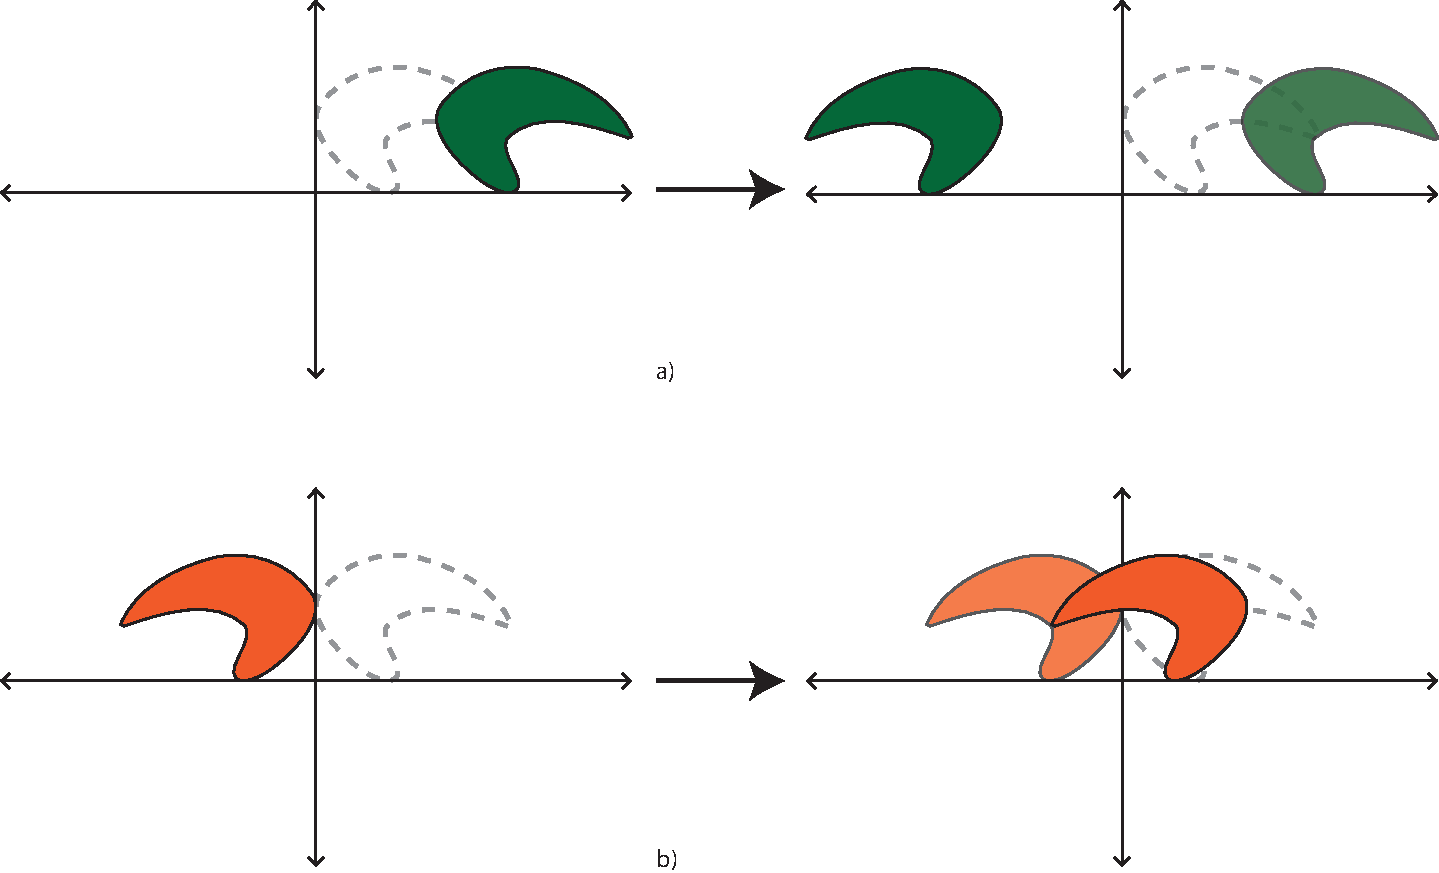
\includegraphics[width=\textwidth]{shiftReflectNotCommuting}
\caption{A simple demonstration that shifts and reflects do not commute in general. a) shows an object with a dashed outline that is translated to the right, and then reflected across the vertical, while b) shows the same object reflected before it is translated to the right. Notice that the final positions of the object are not the same.}\label{fig:notabelian}
\end{figure}

\begin{figure}[t!]
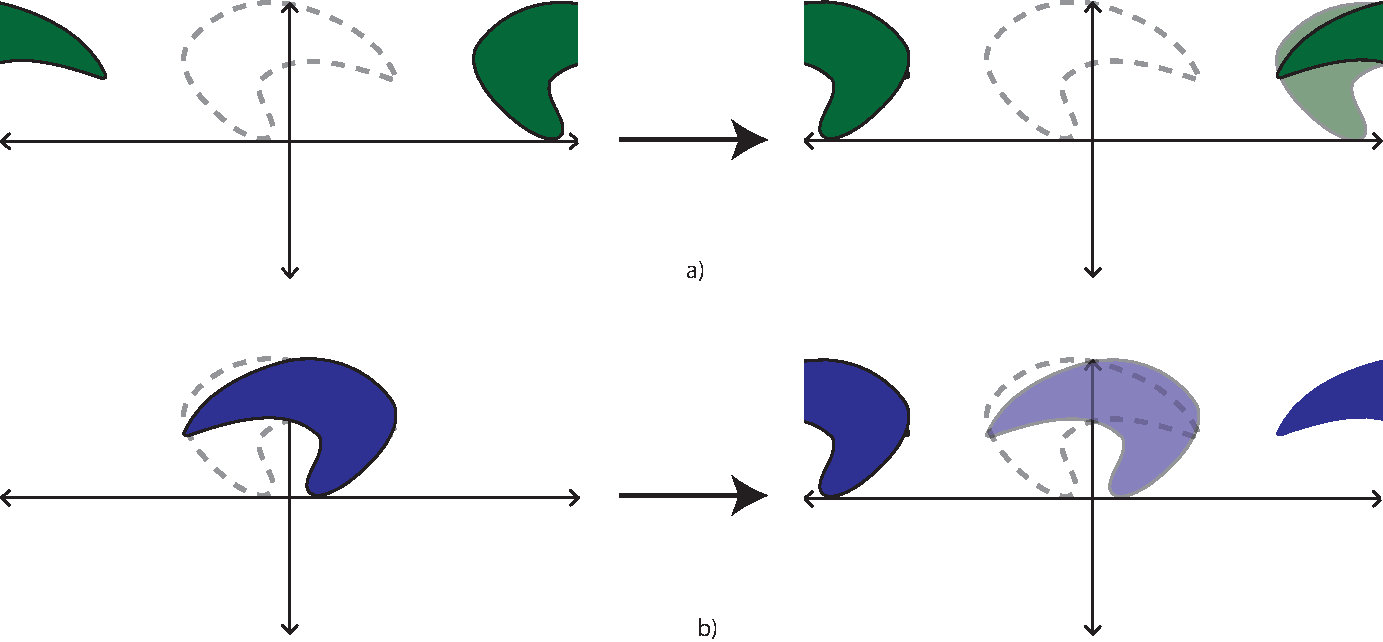
\includegraphics[width=\textwidth]{shiftReflectCommuting}
\caption{When periodic boundary conditions are imposed and translations are fixed to half-period lengths, shifts and reflects commute. a) shows an object that is shifted and then reflected across the vertical, while b) shows the same object reflected across the vertical and then shifted. Notice that the final positions are the same, even if the intermediaries are not.}\label{fig:abelian}
\end{figure}
  
